\documentclass[11pt]{article}

\usepackage[margin=1in]{geometry}
\usepackage{amsfonts}
\usepackage{graphicx}
\usepackage{algorithm}
\usepackage[noend]{algpseudocode}
\usepackage{url}
\usepackage{multirow}

\usepackage[style=authoryear,maxbibnames=5,mincitenames=1,maxcitenames=1]{biblatex}
\renewbibmacro{in:}{%
  \ifentrytype{article}{}{%
  \printtext{\bibstring{in}\intitlepunct}}}
\addbibresource{recomb.bib}

\begin{document}

\title{Cloudbreak: A MapReduce Algorithm for Detecting Genomic Structural Variation from Complete Paired-End Sequence Data Sets}

\author{Christopher W. Whelan \and Kemal S\"onmez}

\maketitle

\begin{abstract}
The detection of genomic structural variations remains one of the the most difficult challenges in analyzing high-throughput sequencing data. Recent approaches have demonstrated that considering multiple mappings of all reads, rather than only uniquely mapped discordant fragments, can improve the performance of read-pair based methods. However, the computational requirements for storing and processing data sets with multiple mappings can be formidable. Meanwhile, the growing size and number of sequencing data sets has led to intense interest in distributing computations to cloud or commodity servers. MapReduce is becoming a standard framework for distributing computation across such compute clusters. We describe a conceptual framework for structural variation detection algorithms in MapReduce based on computing local features along the genome. We demonstrate an implementation of a deletion-finding algorithm in this framework based on fitting a Gaussian mixture model to the distribution of mapped insert sizes spanning each location in the genome. On simulated and real data sets, our approach achieves performance equal to or better than a variety of popular structural variation detection algorithms, including read-pair, split-read, and hybrid approaches, and performs well across a wide range of deletion sizes. In particular, our algorithm excels at discovering deletions of size 40bp-100bp in repetitive regions of the genome. Our implementation is available at \url{http://github.com/cwhelan/cloudbreak}.
\end{abstract}

\newpage

\section{Introduction}

Genomic structural variations such as deletions, insertions, and inversions of DNA, are widely prevalent in human populations and account for the majority of the bases that differ among normal human genomes \autocite{Mills:2011p1611, Conrad:2010ja}. However, detection of structural variations with current high-throughput sequencing technology remains a difficult problem, with limited concordance between available algorithms and high false discovery rates \autocite{Mills:2011p1611}.

Popular SV detection algorithms use three main signals present in high-throughput sequencing data sets. See \textcite{Alkan:2011p547} for a review. Read-pair (RP) based methods use the distance between and orientation of the mappings of the sequenced ends of DNA fragments to identify the signatures of SVs \autocite{Campbell:2008p539,Chen:2009p3,Hormozdiari:2009p284,Sindi:2009gu,Korbel:2009dy}. Traditionally, this involves separating mappings into those that are \emph{concordant} or \emph{discordant}, where discordant mappings deviate from the expected insert size or orientation of the fragment, and then clustering the discordant mappings to find SVs with support from multiple pairs. Read-depth (RD) approaches, in contrast, consider the distribution of concordantly mapped reads to infer the presence of SVs from the depth of coverage of locations along the genome \autocite{Abyzov:2011bk,Alkan:2009cr,Yoon:2009kb,Chiang:2009di}. Finally, split-read (SP) methods look for breakpoints within individual reads by mapping portions of the read to different genomic locations \autocite{Wang:2011p1607,Ye:2009p2}.

RP methods have begun to consider larger and larger data sets. Although the first RP methods used only unambiguously, discordantly mapped read pairs in their analyses, it has been demonstrated that including multiple mappings of discordant read pairs in their analysis improves sensitivity in repetitive and hard-to-map regions of the genome \autocite{Hormozdiari:2009p284,Quinlan:2010gf}. More recently, several RP approaches have considered concordant read pairs, either to integrate RD signals for improved sensitivity and specificity \autocite{Sindi:2012kk,Michaelson:2012fj,Chiara:2012ey}, or to eliminate the thresholds necessary to separate concordant from discordant mappings and be able to detect smaller events \autocite{Marschall:2012ek}. Even so, however, most methods use only a limited number of ambiguous discordant mappings per read pair, because of the storage and computational requirements necessary to process all or most ambiguous mappings of each read pair in a high-coverage data set.

Google's MapReduce \autocite{Dean:2008p277} and its open-source implementation Hadoop\footnote{\url{http://hadoop.apache.org/}}, are designed to manage the storage and efficient processing of very large scale data sets across clusters of commodity servers. Use of the Hadoop framework has been demonstrated for sequencing-related bioinformatic tasks including short read mapping, \autocite{Schatz:2009p278} querying variant databases, \autocite{Oconnor:2010p1835} SNP calling, \autocite{Langmead:2009p1225} RNA-seq differential expression analysis, \autocite{Langmead:2010p1268} ChIP-seq peak calling, \autocite{Feng:2011p1228} and computing genome mappability \autocite{Lee:2012bk}. MapReduce requires a specific programming model, however, which can make it difficult to design general-purpose algorithms for arbitrary sequencing analysis problems like SV detection.

In this paper, we describe a framework for solving SV detection problems in Hadoop and MapReduce based on the computation of local features along the genome from paired end mappings. We then demonstrate an implementation of an SV algorithm, Cloudbreak, for discovering genomic deletions, which computes local features based on the insert sizes of spanning mapping. Cloudbreak computes features that build on the ideas of \autocite{Lee:2009da}, who modeled the distribution of insert sizes at each genomic location as a Gaussian Mixture Model (GMM). We then characterize our algorithm's performance on simulated and real data sets.

\section{Results}\label{results}

\subsection{A MapReduce Framework for SV Detection Algorithms}

The MapReduce programming model \autocite{Dean:2008p277} divides computation across a cluster into three phases. In the first phase, \emph{mappers} developed by the application programmer examine small blocks of data and emit a set of $\langle key, value \rangle$ pairs for each block examined. The MapReduce framework then sorts the output of the mappers by key, and aggregates all values that are associated with each key. Finally, the framework executes \emph{reducers}, also created by the application developer, which process all of the values for a particular key and produce one or more outputs that summarize or aggregate those values. Hadoop is an open source project of the Apache Foundation which provides an implementation of the MapReduce programming framework as well as a distributed file system for storing large data sets across a cluster. In addition to a MapReduce programming framework, Hadoop also provides a distributed file system (HDFS), which facilitates storing large data sets redundantly across a cluster. MapReduce and Hadoop allow efficient processing of large data sets by scheduling tasks for execution as close as possible to the nodes which hold the required data, minimizing network traffic and I/O contention.

The need to separate logic into mappers and reducers makes it difficult to implement traditional read-pair approaches in MapReduce. This is especially true because of the graph data structures and global clustering of paired end mappings at the heart of many read-pair approaches. MapReduce algorithms, by contrast, excel at conducting many independent calculations in parallel. In genomic sequencing applications, for example, MapReduce based SNP-callers Crossbow \autocite{Langmead:2009p1225} and GATK \autocite{McKenna:2010p1051} perform independent calculations for each location or partition in the genome. The RP-based SV callers MoDIL \autocite{Lee:2009da} and forestSV \autocite{Michaelson:2012fj} attempt to solve the SV detection problem by computing scores or features at varying locations along the genome and then integrating those features into SV predictions in a post-processing step. Here we show that this formulation can be easily translated to the MapReduce programming model.

Our formulation divides processing into two distinct MapReduce jobs. The first job finds possible alignment locations for pairs of reads in FASTQ format. The second job computes features from the set of reads that are relevant to each of a set of small intervals covering the genome. In the final stage, the features for each location are exported from the Hadoop file system and post-processed to produce a set of SV calls which span multiple genomic intervals. The MapReduce algorithm is summarized below with a detailed explanation following.

\algrenewcommand\algorithmicprocedure{\textbf{job}}
  \begin{algorithmic}[1]
    \Procedure{Alignment}{}
    \Function{Map}{$\textrm{ReadPairId }rp, \textrm{ReadId }r, \textrm{ReadSequence }s, \textrm{ReadQuality }q$}
    \ForAll{$ \textrm{Alignments }a \in \textrm{Align}(<s,q>)$}
    \State $\textsc{Emit}(\textrm{ReadPairId }rid, \textrm{Alignment }a)$
    \EndFor
    \EndFunction
    \Function{Reduce}{$\textrm{ReadPairId }rid, \textrm{Alignments }a_{1,2,\ldots}$}
    \State $\textrm{AlignmentPairList }ap \gets \textrm{ValidAlignmentPairs}(a_{1,2,\ldots}$
    \State $\textsc{Emit}(\textrm{ReadPairId }rp, \textrm{AlignmentPairList} ap)$
    \EndFunction
    \EndProcedure

    \Procedure{Compute SV Features}{}
    \Function{Map}{$\textrm{ReadPairId }rp, \textrm{AlignmentPairList }ap$}
    \ForAll{$ \textrm{AlignmentPairs }<a_1,a_2> \in ap$}
    \State $ \textrm{ReadPairInfo }spi \gets <\textrm{InsertSize}(a_1,a_2), \textrm{AlignmentScore}(a_1,a_2)>$
    \ForAll{$ \textrm{GenomicLocations }l \in \textsc{Loci }(a_1,a_2)$}
    \State $\textsc{Emit}(\textrm{GenomicLocation }l, \textrm{SpanningPairInfo }spi)$
    \EndFor
    \EndFor
    \EndFunction
    \Function{Reduce}{$\textrm{GenomicLocation }l, \textrm{ReadPairInfos }spi_{1,2,\ldots}$}
    \State $\textrm{SVFeatures } \phi_l \gets \Phi(\textrm{InsertSizes }i_{1,2,\ldots}, \textrm{AlignmentScores }q_{1,2,\ldots})$
    \State $\textsc{Emit}(\textrm{GenomicLocation }l, \textrm{SVFeatures } \phi_l)$
    \EndFunction
    \EndProcedure
    \State $\textrm{StructuralVariationCalls } sv \gets \textsc{PostProcess }(\Phi)$ 
  \end{algorithmic}

The alignment job uses sensitive alignment tools and settings to discover as many mapping locations for each read pair as possible. In the mapping phase, mappers align reads in single-end mode to the reference genome in parallel, outputting each possible mapping location as a value under a key identifying the read pair. In the reduce phase, Cloudbreak combines pairs of mapping locations for the two ends of a read pair to produce all possible combinations of mapping locations found. Our algorithm could use any aligner that is capable of reporting multiple alignments for reads. We report results generated with alignments from RazerS 3 \autocite{Weese:2012by}, which in our tests displayed the best combination of sensitivity, performance, and memory usage suitable for parallelization in Hadoop. Our implementation also contains wrappers to execute the aligners Novoalign\footnote{\url{http://wwww.novocraft.com}}, mrFAST \autocite{Alkan:2009cr}, and Bowtie 2 \autocite{Langmead:2012jh}, as well as the ability to import a pre-aligned BAM file directly to HDFS.

In the second job, we compute a set of features for each location in the genome. To begin, we tile the genome with small fixed-width, non-overlapping intervals. For the experiments reported in this paper we use an interval size of 25bp. Let $L = \left\{l_1,l_2,\ldots,l_N\right\}$ be the set of intervals covering the entire genome. Let $R_1 = \left\{r_{1,1},r_{1,2},\ldots,r_{1,M}\right\}$ and $R_2 = \left\{r_{2,1},r_{2,2},\ldots,r_{2,M}\right\}$ be the input set of paired reads. Let $A^1 = \left\{a^{1}_{m,1},a^{1}_{m,2},\ldots,a^{1}_{m,K}\right\}$ and $A^2 = \left\{a^{2}_{m,1},a^{2}_{m,2},\ldots,a^{2}_{m,K}\right\}$ be the set of alignments for the left and right reads from read pair $m$. For any given pair of alignments of the two reads in a read pair $a^{1}_{m,i}$ and $a^{2}_{m,j}$, let the $\textrm{ SpanningPairInfo} spi_{m,i,j}$ be information about the pair relevant to detecting SVs, e.g. the fragment size implied by the alignments and the likelihood the alignments are correct. We define three functions, $\textsc{Loci } : \langle a^{1}_{m,i},a^{2}_{m,j} \rangle \rightarrow L_m \subseteq L$, $\Phi : \left\{\textrm{SpanningPairInfo }spi_{m,i,j}\right\} \rightarrow \mathbb{R}^N$, and $\textsc{PostProcess}$, which maps features across the genome into a set of SV calls. The first maps an alignment to a set of genomic locations to which it is relevant for SV detection; for example, the set of locations overlapped by the internal insert implied by the read alignments. We optimize this step by assuming that if there exist concordant mappings for a read pair, defined as those where the two alignments are in the proper orientation and with an insert size within three standard deviations of the expected library insert size, one of them is likely to be correct and therefore we do not consider any discordant alignments of the pair. The second function maps a set of SpanningPairInfos relevant to a given location to a real-valued vector of features useful for SV detection. 

We describe one possible set of functions below; however, we believe that there are many possible mappings that would be useful for different types of SV detection problems that vary in event type sought, depth of coverage, heterogeneity of the sample, etc.

\subsection{Cloudbreak: A Hadoop Deletion Detection Implementation}

We have implemented a deletion detection algorithm for medium-to-high coverage diploid samples in this framework called Cloudbreak. 
\begin{description}
\item[\sc{Loci}] Because we are detecting deletions, we map SpanningPairInfo from each possible alignment to the genomic locations overlapped by the implied internal insert between the reads. For efficiency, we define a maximum detectable deletion size of 25,000bp, and therefore alignment pairs which map more than 25kb apart, or in the incorrect orientation, to no genomic locations.
\item[$\Phi$] To compute features for each genomic location, we follow \textcite{Lee:2009da}, who observed that if all mappings are correct, the insert sizes implied by mappings which span a given genomic location should follow a Gaussian mixture model (GMM) whose parameters depend on whether a deletion or insertion is present at that locus. Briefly: if there is no indel, the insert sizes implied by spanning alignment pairs should follow the distribution of actual fragment sizes in the sample, which is typically modeled as normally distributed with mean $\mu$ and standard deviation $\sigma$. If there is a homozygous deletion or insertion of length $l$ at the location, $\mu$ should be shifted to $\mu + l$, while $\sigma$ will remain constant. Finally, in the case of a heterozygous event, the distribution of insert sizes will follow a mixture of two normal distributions, one with mean $\mu$, and the other with mean $\mu + l$, both with an unchanged standard deviation of $\sigma$, and mixing parameter $\alpha$ that describes the relative weights of the two components. Because the mean and standard deviation of the fragment sizes are selected by the experimenter and therefore known \emph{a priori} (or at least easily estimated based on a sample of alignments), we only need to estimate the mean of the second component at each locus, and the mixing parameter $\alpha$.

To handle incorrect and ambiguous mappings, we assume that in general they will not form normally distributed clusters in the same way that correct mappings will, and therefore use an outlier detection technique to filter the observed insert sizes for each location. We rank the observed insert sizes and define as an outlier an observation whose $k$th nearest neighbor is more than $n\sigma$ distant, where $k = 3$ and $n = 5$. In addition, we rank all observations by the estimated probability that the mapping is correct and use an \emph{adaptive quality cutoff} to filter observations: we discard all observations where the estimated probability the mapping is correct is less than the score of the maximum quality observation minus a constant $c$. This allows the use of more uncertain mappings in repetitive regions of the genome while restricting the use of low-quality mappings in unique regions.

We fit the means and of the GMM using the Expectation-Maximization algorithm. Let $Y = y_{1,2, \ldots m}$ be the observed insert sizes at each location after filtering, and the library to have mean fragment size $\mu$ with standard deviation $\sigma$. We initialize the two components to have means $\mu$ and $\bar{Y}$ and standard deviation $\sigma$, and set $\alpha = .5$. In the E step, we compute for each $y_i$ and GMM component $j$ the value $\gamma_{i,j}$, which is the normalized likelihood that $y_i$ was drawn from component $j$. We also compute $n_j = \sum_i{\gamma_{i,j}}$, the relative contributions of the data points to each of the two distributions. In the M step, we update $\alpha$ to be $n_2 - \left|Y\right|$, and set the mean of the second component to be $\sum_m{\gamma_{m,2} + y_m}$. We repeat E and M steps until convergence or a maximum number of steps has been taken.

Our features for each location $l$ include the log-likelihood ratio of the filtered observed data points under the fit GMM to their likelihood under the distribution $N(\mu,\sigma)$, the final value of the mixing parameter $\alpha$, and $\mu'$, the estimated mean of the second GMM component.

\item[\sc{PostProcess}] We convert our features along the genome to deletion calls by first extracting contiguous genomic loci where the log-likelihood ratio of the two models is greater than a given threshold. To eliminate noise we apply a median filter with window size 5. We end regions when $\mu'$ changes by more than 60bp, discard regions where the average value of $\mu'$ is less than $\mu$ or where the length of the region differs from $\mu'$ by more than $\mu$.
\end{description}


\section{Results}\label{results}

We compared the performance of Cloudbreak for detecting deletions to a selection of popular tools: the RP methods Breakdancer \autocite{Chen:2009p3} and GASVPro, \autocite{Sindi:2012kk}, the SR method Pindel \autocite{Ye:2009p2}, and the hybrid RP-SR method DELLY. \autocite{Rausch:2012he} In each case we use default parameters and attempt to follow the recommend pipelines for alignment for each tool (See Methods for details).

We use the following criteria to define a true prediction given a gold standard set of deletions to test against: A predicted deletion is counted as a true positive if a) it overlaps with a deletion from the gold standard, b) the length of the predicted call is within 300bp (the library fragment size in both our real and simulated libraries) of the length of the true deletion, and c) the true deletion has not been discovered by another prediction from the same method. Furthermore, we find that Pindel is very accurate at discovering deletions less than or equal to 40bp in length, so we exclude from consideration calls that match a true deletion of less than 40bp where the call is less than or equal to 75bp in length. It should be noted that the methods tested here vary in their breakpoint resolution: SR methods have higher resolution than RP methods. Cloudbreak sacrifices additional resolution (by dividing the genome into 25bp windows); we strive however to increase sensitivity and specificity in the hopes that such calls could still be useful even if their resolution is limited. This seems reasonable to us given the possibility of pipelines in which RP calls are refined by SR mappings or local assembly methods.

\subsection{Tests with Simulated Data}

As has been observed elsewhere, there is no available test set of real Illumina sequencing data from a sample that has a complete annotation of structural variations from the reference. Therefore, testing with simulated data is important to fully characterize an algorithm's performance characteristics. On the other hand, it is important that the simulated data contain realistic SVs that follow patterns of SVs observed in real data. To address this, we took one of the most complete lists of SVs from a single sample available, the list of homozygous deletions from the genome of J. Craig Venter \autocite{Levy:2007fb}. Since there are relatively few heterozygous deletions annotated in that set, we randomly assigned each deletion to be either homozygous or heterozygous and applied them to one or both of two copies of the human GRCh36 chromosome 2 reference sequence. We then simulated paired Illumina reads from these modified references using \emph{dwgsim} from the DNAA software package\footnote{\url{http://sourceforge.net/apps/mediawiki/dnaa/}}. We simulated 100bp reads with a mean fragment size of 300bp and a standard deviation of 30bp, and generated 15X coverage for each modified sequence. Pooling the reads from both simulations gives 30X coverage for a diploid sample with a mix of homozygous and heterozygous deletions.

\begin{figure}[t]
\centering
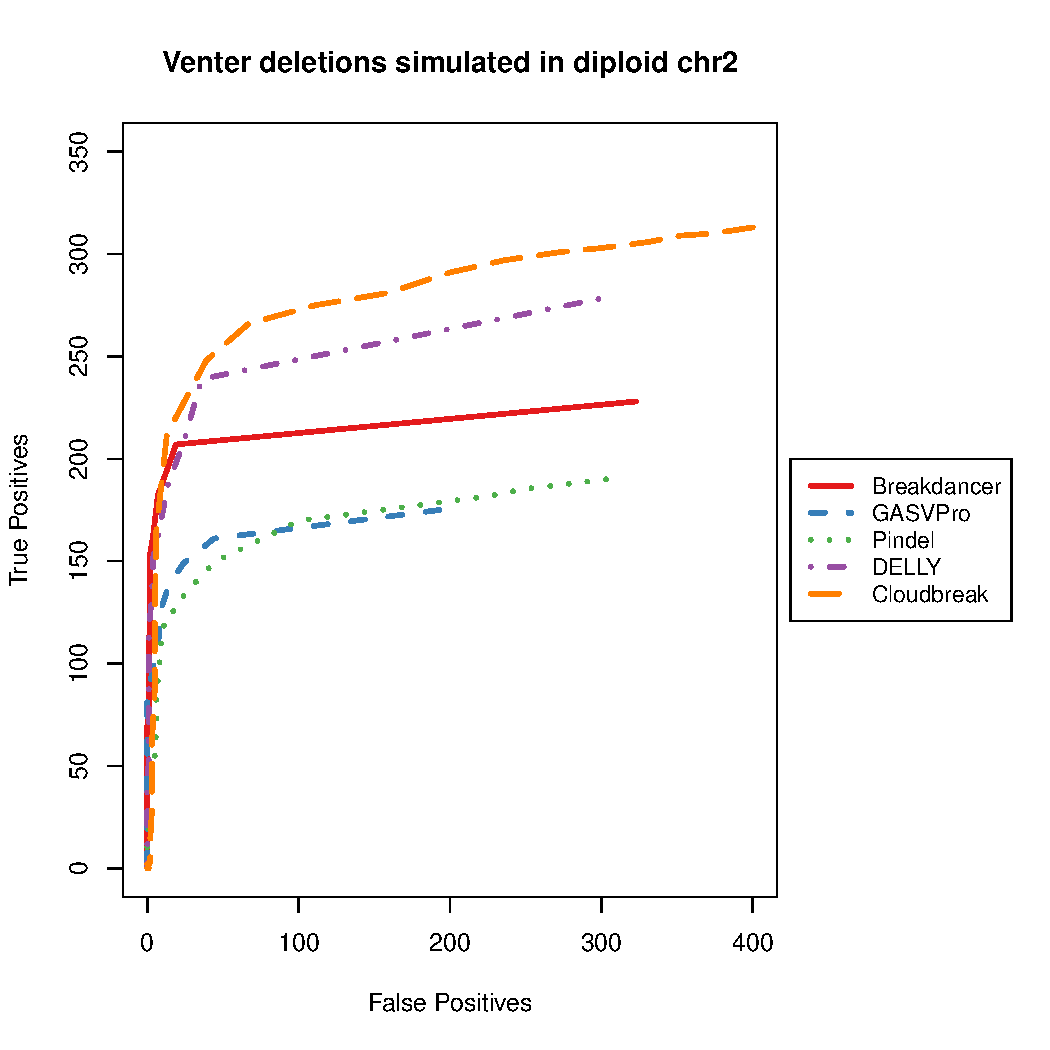
\includegraphics[width=0.6\textwidth]{CHR2SIM_ROC_NEW.pdf}
\caption{ROC curve of deletion prediction performance on a simulated set of reads giving diploid coverage of 30X on human chromosome 2 with deletions from the Venter genome added to one or both haplotypes. Thresholds vary by: Cloudbreak - likelihood ratio; Breakdancer - score; DELLY, GASVPro, and Pindel - number of supporting read pairs.}
\label{chr2roc}
\end{figure}

Figure \ref{chr2roc} shows an ROC plot of the performance of each algorithm on the simulated data set. All approaches show excellent specificity at high thresholds in this simulation. Cloudbreak and DELLY provide the greatest sensitivity at high specificity. Table \ref{chr2preds} shows the total number of simulated deletions found by each tool when using choosing a threshold that gives an FDR of 0.1 based on the ROC curve, representing cutoffs of 1.68 log likelihood ratio for Cloudbreak, score 44 for Breakdancer, 8 supporting read pairs for GASVPro, four supporting read pairs for DELLY, and 18 supporting read pairs for Pindel. Cloudbreak shows excellent sensitivity at each size class, and contributes a number of exclusive true predictions in both small and medium size classes. In addition, Cloudbreak has the greatest sensitivity to repeats that intersect RepeatMasker annotated regions of the reference sequence, correctly identifying 12\% more repeat-overlapping deletions than the nearest competitor.

\begin{table}[b]
\begin{center}
\begin{tabular}{rrrrrr}
  \hline
 & 40-100bp  & 101-250bp  & 251-500bp & 501-1000bp & $>$ 1000bp \\ 
 Total Number & 219 & 82 & 81 & 31 & 26 \\ 
  \hline
Cloudbreak &  \textbf{87} (12) &  56 (0) &  \textbf{61} (\textbf{4}) &  \textbf{10} (1) &  \textbf{16} (0) \\ 
  Breakdancer &  73 (11) &  58 (1) &  54 (0) &  7 (0) &  15 (0) \\ 
  GASVPro &  46 (3) &  27 (0) &  47 (1) &  5 (\textbf{2}) &  13 (0) \\ 
  DELLY &  61 (7) &  \textbf{66} (\textbf{4}) &  56 (0) &  9 (0) &  \textbf{16} (0) \\ 
  Pindel &  52 (\textbf{14}) &  11 (0) &  37 (0) &   4 (0) &  14 (0) \\ 
   \hline
\end{tabular}
\end{center}
\caption{The number of simulated deletions in the 30X diploid chromosome 2 with Venter deletions found by each tool at a 10\% FDR, as well as the number of those deletions that were discovered exclusively by each tool (in parentheses). The total number of deletions in each size class in the true set of deletions is shown in the second row of the header.}
\label{chr2preds}
\end{table}

\subsection{Tests with Biological Data}

We downloaded a data set of reads taken from a DNA sample of Yoruban individual NA18507, experiment ERX009609 from the Sequence Read Archive.\footnote{\url{http://sra.dnanexus.com/experiments/ERX009609}} This sample was sequenced on the Illumina Genome Analyzer II platform using with 100bp paired end reads and a mean fragment size (minus adapters) of 300bp, with a standard deviation of 15bp. The sample was sequenced to a depth of approximately 37X coverage.

To create a gold standard set of deletions to test against, we pooled annotated deletions discovered by three previous studies on the same sample. These included data from the Human Genome Structural Variation Project\footnote{\url{http://hgsv.washington.edu/general/download/SNPs_DIPs/}} reported by \textcite{Kidd:2008p926}, a survey of small indels conducted by \textcite{Mills:2011fi}, and deletions from the merged call set of the phase 1 release of the 1000 Genomes Project \autocite{GenomesProjectConsortium:2012co} which were genotyped as present in NA18507. We merged any overlapping calls into the region spanned by their unions. It should be noted that the 1000 Genomes call set was partially produced using DELLY and Breakdancer, and therefore those calls are ones that those tools are sensitive to.

\begin{figure}[t]
\centering
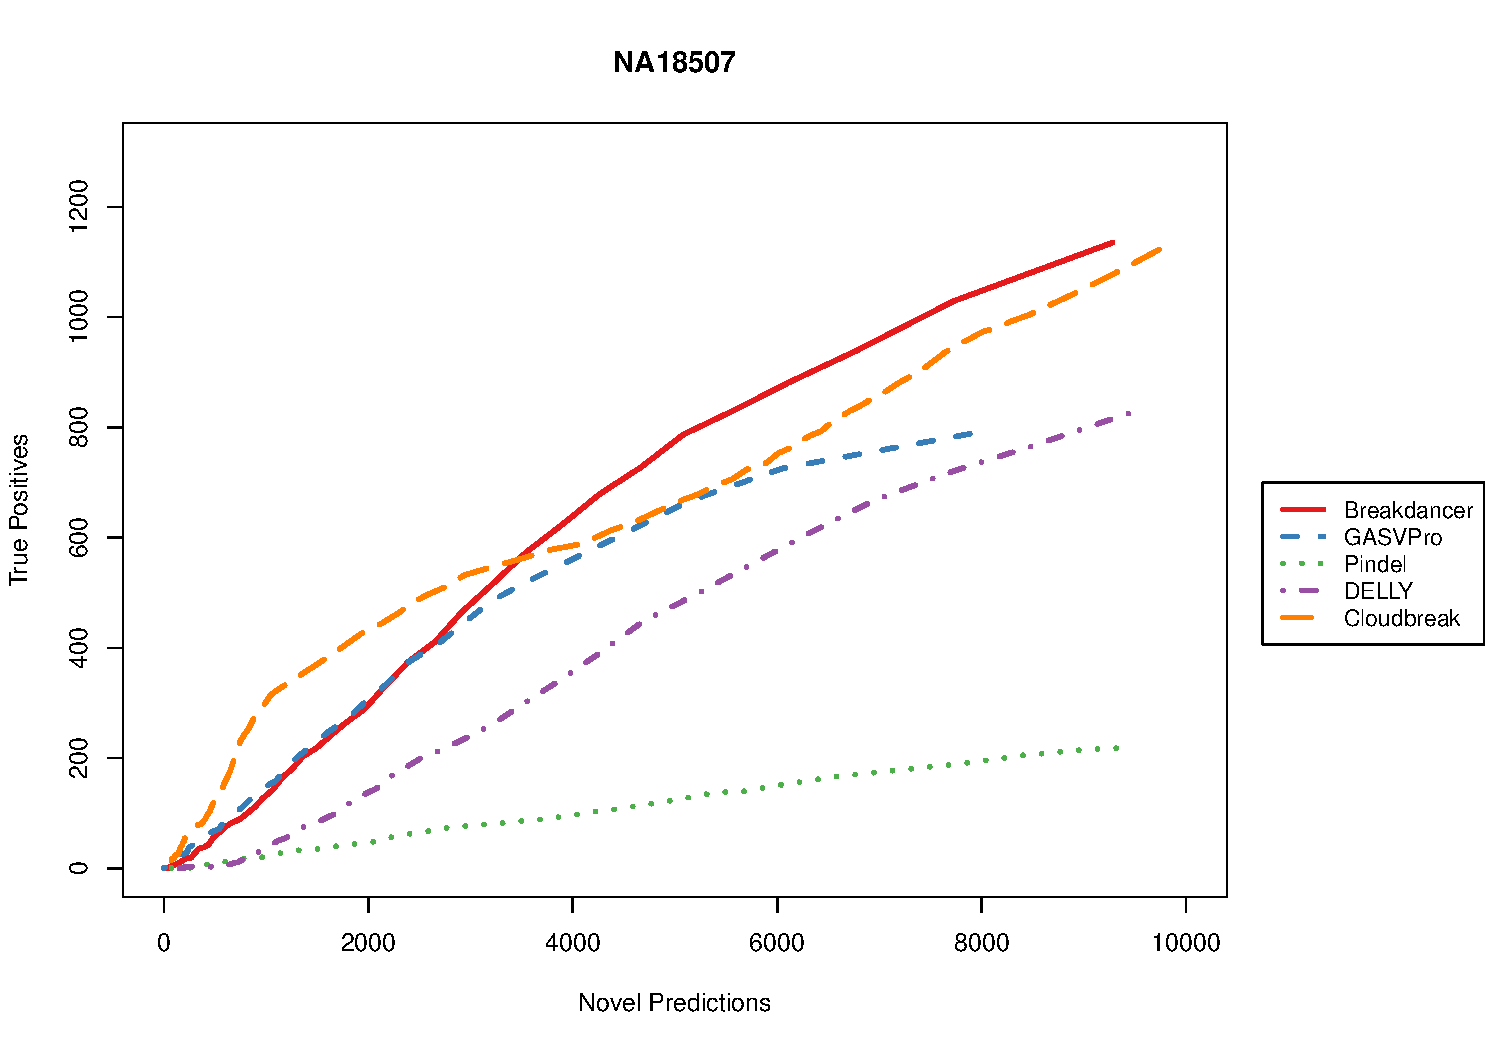
\includegraphics[width=0.75\textwidth]{NA18507_ROC.pdf}
\caption{ROC curve of deletion prediction performance on the 37X NA18507 sample, test against the combined gold standard deletion set taken from \textcite{Kidd:2008p926}, \textcite{Mills:2011fi}, and \textcite{GenomesProjectConsortium:2012co}.}
\label{NA18507roc}
\end{figure}

Figure \ref{NA18507roc} shows the performance of each algorithm on the NA18507 data set when compared against the gold standard deletion set, using the same rules for a match as described in the previous section. All algorithms show far less specificity for the gold standard set than they did for the true deletions in the single chromosome simulation, although it is difficult to tell how much of the difference is due to the added complexity of real data and a whole genome, and how much is due to the missing deletions in the gold standard set. 

We then tested the predictions made by each algorithm using the same cutoffs that yielded a 10\% FDR on the simulated chromosome 2 data set, adjusted for the difference in coverage from 30X to 37X. The precision and recall with respect to the gold standard deletion set, as well as the performance of each algorithm at predicting each size class at those cutoffs, is shown in Table \ref{NA18507preds}. Although Cloudbreak is not the top performer in any category, it is the second-best in every category and provides a large number of exclusive predictions.

% latex table generated in R 2.15.2 by xtable 1.7-0 package
% Tue Jan  1 22:36:02 2013
\begin{table}[t]
\begin{center}
\begin{tabular}{rrr|rrrrr}
  \hline
 & Prec. & Recall & 40-100bp & 101-250bp & 251-500bp & 501-1000bp & $>$ 1000bp \\ 
Total Number & & & 9,980 & 242 & 218 & 110 & 375 \\
  \hline
Cloudbreak & 0.094 & 0.115 & 601 (201) & 142 (8) & 171 (\textbf{7}) &  87 (\textbf{2}) & 254 (\textbf{7}) \\ 
Breakdancer & 0.118 & 0.094 & 337 (31) & 137 (4) & 169 (0) & 93 (0) & 293 (2) \\
  GASVPro & \textbf{0.127} & 0.048 & 189 (39) &  42 (1) & 102 (1) &  41 (0) & 147 (0) \\ 
  DELLY & 0.070 & 0.091 & 260 (15) & \textbf{156} (\textbf{13}) & \textbf{176} (5) &  \textbf{94} (0) & \textbf{304} (4) \\ 
  Pindel & 0.024 & \textbf{0.130} & \textbf{1,039} (\textbf{791}) & 51 (0) & 125 (1) &  53 (0) & 149 (1) \\ 
   \hline
\end{tabular}
\end{center}
\caption{The precision and recall with respect to the gold standard set of each tool on the NA18507 data set, as well as the number of deletions in the gold standard set of each size class found by each tool. The same cutoffs were used as for the simulated data, adjusted for the difference in coverage.}
\label{NA18507preds}
\end{table}

\subsection{Performance in Repetitive Areas}

We analyzed the predictions made by Cloudbreak to determine whether any particular class of deletion event was contributing to its performance. We found that Cloudbreak shows particularly strong performance in detecting deletions that overlap RepeatMasker-annotated elements (Table \ref{repmaskpreds}) in both the simulated and NA18507 data sets, especially compared to the RP-based methods. Since deletions and other SVs are enriched in repetitive regions of the genome in both of our data sets, this contributes highly to Cloudbreak's performance, and demonstrates the value in considering as many possible mappings of ambiguously mapping reads as possible.

\begin{table}
\begin{center}
\begin{tabular}{rrr|rr}
 & \multicolumn{2}{c}{Simulated Data} & \multicolumn{2}{c}{NA18507} \\
\hline
 &  Non-repeat & Repeat  &  Non-repeat & Repeat \\ 
 Total Number & 122 & 317 & 604 & 10,321 \\ 
  \hline
Cloudbreak & \textbf{36} (5) & \textbf{194} (\textbf{12}) & \textbf{251} (\textbf{34}) & 1,004 (191) \\ 
  Breakdancer &  33 (3) & 174 (9) & 208 (12) & 821 (25) \\ 
  GASVPro & 20 (2) & 118 (4) & 93 (5) & 428 (36) \\ 
  DELLY & 35 (\textbf{6}) & 173 (5) & 229 (23) & 761 (14) \\ 
  Pindel & 12 (5) & 106 (9) & 148 (\textbf{31}) & \textbf{1,269} (\textbf{762}) \\ 
   \hline
\end{tabular}
\end{center}
\caption{True positive deletions on the simulated and NA18507 data sets identified by each tool, broken down by whether or not the deletion overlaps with a RepeatMasker-annotated repetitive element.}
\label{repmaskpreds}
\end{table}

\subsection{Genotyping Deletions}

Since Cloudbreak explicitly fits a mixture of insert size distributions at each location, and each component of the mixture represents an allele containing or not containing a deletion, it should be possible to use the parameters of the fit GMM to infer the genotype of each predicted variant, assuming that our pipeline is capturing all relevant read mappings near the locus of the variant. To test this, we attempted to classify true positive Cloudbreak deletion predictions from the sets described above for both the simulated and biological data sets. Because we simulated a diploid genome, we had genotypes for the simulated data readily available. For the real dataset, we only considered the deletions from the 1000 Genomes Project data set, which had been genotyped as part of the Phase 1 release using the population-scale SV detection algorithm Genome STRiP \autocite{Handsaker:2011ki}. We found that we could use $\alpha$, the mixing parameter that controls the weight of the two components in the GMM, to accurately predict deletion genotypes. By setting a simple cutoff of .2 on the average value of $\alpha$ in each Cloudbreak prediction, we were able to achieve 87.8\% and 95.7\% accuracy in predicting the genotype of the true positive deletions we detected in the simulated and real data sets, respectively. Table \ref{genotypeaccuracy} shows confusion matrices for the two samples using this simple classifier.

\begin{table}
\begin{center}
\begin{tabular}{r|r|rr|rr|}
\multicolumn{2}{c}{}  & \multicolumn{4}{c}{Actual Genotypes} \\
\multicolumn{2}{c}{}  & \multicolumn{2}{c}{Simulated Data} & \multicolumn{2}{c}{NA18507} \\
\cline{3-6}
\multicolumn{2}{c|}{} &  Homozygous & Heterozygous & Homozygous & Heterozygous \\ 
\cline{2-6}
\multirow{2}{*}{\shortstack{Predicted \\ Genotypes}} & Homozygous & 129 & 4 & 77 & 12 \\
 & Heterozygous & 24 & 73 & 4 & 280 \\
\cline{2-6}
\end{tabular}
\end{center}
\caption{Confusion matrices for the predicted genotype of deletions found by Cloudbreak on both the simulated and NA18507 data sets.}
\label{genotypeaccuracy}
\end{table}


\section{Methods}\label{discussion}

Cloudbreak is a native Java Hadoop application. We deployed Cloudbreak on a 56-node cluster running the Cloudera CDH3 Hadoop distribution, version 0.20.2-cdh3u4, with snappy compression enabled.

For each evaluated SV detection program we attempt to follow the recommended alignment pipeline. Simulated reads were aligned to hg18 chromosome 2. Cloudbreak alignments were executed in parallel using Hadoop tasks which wrap RazerS 3 version 3.1, with parameters \verb|-rr 99 -i 94 -m 1000|, requesting 99\% sensitivity, a maximum edit distance between read and reference of 6\%, and up to 1000 possible alignments reported for each read. Alignments for the other programs were first aligned using BWA \autocite{Li:2009p836} version 0.6.2-r126, with parameter \verb|-e 5| to allow for longer gaps in alignments due to the number of small indels near the ends of larger indels in the Venter data set. GASVPro also accepts ambiguous mappings; we extracted read pairs that did not align concordantly with BWA and re-aligned them with Novoalign V2.08.01, with parameters \verb|-a -r -Ex 1100 -t 250|. 

We ran Breakdancer version 1.1\_2011\_02\_21 by first executing \verb|bam2cfg.pl| and then running \verb|breakdancer_max| with the default parameter values. We ran DELLY version 0.0.9 with the \verb|-p| parameter and default values for other parameters. We ran GASVPro version 1.2 using the GASVPro.sh script and default parameters. Finally, we ran Pindel 0.2.4t with default parameters.

\section{Discussion}\label{conclusions}

\section{Acknowledgements}

We would like to thank Izhak Shafran at the Center for Spoken Language Understanding and Lucia Carbone of the Department of Behavioral Neuroscience for their advice, support, and shared computational resources.

\newpage

\printbibliography

\end{document}

% LocalWords:  Abyzov 2011bk Yoon 2010gf 2012kk Michaelson 2012fj 2012ey Feng
% LocalWords:  Oconnor Langmead RNA-seq Langmead ChIP-seq 2012bk langle textbf
% LocalWords:  algrenewcommand algorithmicprocedure textrm rp textrm textrm ap
% LocalWords:  textrm textsc ldots spi RazerS Weese Novoalign Bowtie 2012jh sc
% LocalWords:  rightarrow subseteq mathbb th 2007fb dwgsim includegraphics rr
% LocalWords:  textwidth haplotypes chr2roc chr2preds rrrrrr hline Yoruban
% LocalWords:  indels NA18507preds printbibliography
